\documentclass[tikz,border=5pt]{standalone}
\usepackage{amsmath}
\usepackage{pgfplots}
\pgfplotsset{compat=1.18}

\definecolor{corba}{HTML}{365FB3}
\definecolor{punt}{HTML}{B91C1C}
\definecolor{assimptota}{HTML}{6B7280}

\begin{document}
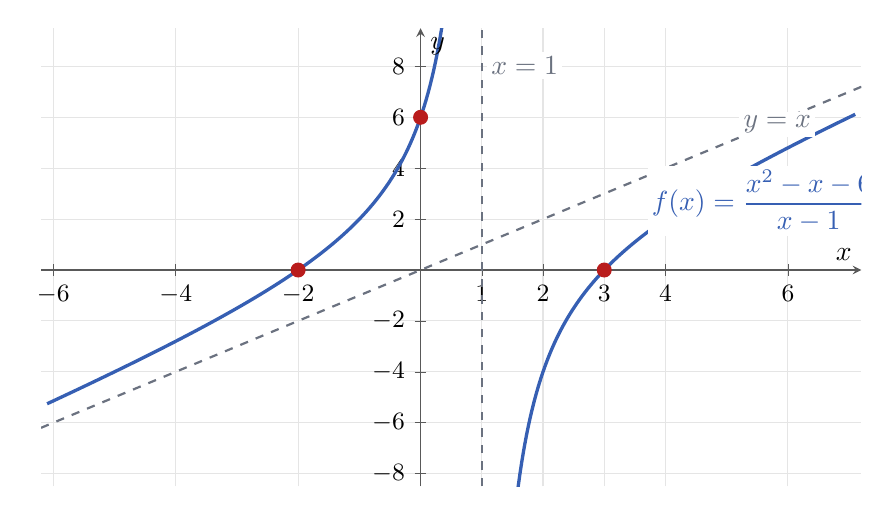
\begin{tikzpicture}
  \begin{axis}[
    width=12cm,
    height=7.4cm,
    axis lines=middle,
    xmin=-6.2,
    xmax=7.2,
    ymin=-8.5,
    ymax=9.5,
    xlabel={$x$},
    ylabel={$y$},
    xtick={-6,-4,-2,0,1,2,3,4,6},
    ytick={-8,-6,-4,-2,0,2,4,6,8},
    grid=major,
    grid style={black!10},
    axis line style={black!65},
    tick style={black!65},
    tick label style={font=\small},
    clip=true,
  ]
    \addplot[assimptota, dashed, thick, domain=-6.2:7.2, samples=2] {x};
    \addplot[assimptota, dashed, thick] coordinates {(1,-8.5) (1,9.5)};

    \addplot[corba, very thick, domain=-6.1:0.78, samples=220]
      {x-6/(x-1)};
    \addplot[corba, very thick, domain=1.22:7.1, samples=220]
      {x-6/(x-1)};

    \addplot[only marks, mark=*, mark size=2.5pt, punt]
      coordinates {(-2,0) (0,6) (3,0)};

    \node[anchor=south west, text=assimptota, fill=white, inner sep=1.5pt]
      at (axis cs:5.2,5.2) {$y=x$};
    \node[anchor=south west, text=assimptota, fill=white, inner sep=1.5pt]
      at (axis cs:1.08,7.5) {$x=1$};
    \node[anchor=south west, text=corba, fill=white, inner sep=1.5pt]
      at (axis cs:3.7,1.3) {$f(x)=\dfrac{x^2-x-6}{x-1}$};
  \end{axis}
\end{tikzpicture}
\end{document}
